% ============================================================
%  htt_base — Final Results Report (credible-claim distillation)
%
%  Self-contained. Final results only; no development history.
%  Separate from the full VER06 manuscript (docs/manuscript/),
%  which is preserved unchanged. This document carries only the
%  results that survive the project's claim-firewall: diagnostic-
%  only framework statements, Wolfram-verified conditional
%  theorems, null-calibrated model-independent real-data
%  measurements, and explicitly transfer-conditional diagnostics.
%
%  Build:  latexmk -pdf main.tex   (run from docs/final_report/)
% ============================================================
\documentclass[11pt,a4paper]{article}

\usepackage{amsmath,amssymb,amsthm}
\usepackage{mathtools}
\usepackage{bm}
\usepackage{booktabs}
\usepackage{array}
\usepackage{graphicx}
\usepackage{xcolor}
\usepackage[hidelinks]{hyperref}
\usepackage{geometry}
\usepackage{microtype}
\usepackage{caption}
\usepackage{enumitem}

\geometry{margin=2.4cm}
\setlength{\emergencystretch}{3em}
\graphicspath{{../../figures/}}

\newcommand{\xC}{x_{C}}
\newcommand{\xmax}{x_{\max}}
\newcommand{\Sigstd}{\Sigma^{2}_{\mathrm{std}}}
\newcommand{\Wstd}{W^{2}_{\mathrm{std}}}
\newcommand{\Otilt}{\Omega_{\mathrm{tilt}}}
\newcommand{\Okaniso}{\Omega_{k,\mathrm{aniso}}}
\newcommand{\Fshear}{F_{\mathrm{shear}}}
\newcommand{\GF}{G_{F}}

\theoremstyle{plain}
\newtheorem{theorem}{Theorem}
\theoremstyle{definition}
\newtheorem{definition}{Definition}

\title{\textbf{Tetrad-Based Departure Decomposition for FLRW Anisotropy}\\[4pt]
\large Final Results Report --- Credible-Claim Distillation}
\author{BASS / HTT / MIO / OBSSTAT stack\\\small Soongsil OMEG Institute}
\date{Compiled \today}

\begin{document}
\maketitle

\begin{abstract}
\noindent
This report distills the \emph{credible, defensible} results of the
tetrad-based departure-decomposition program into a single
self-contained document. It deliberately excludes development
history, superseded paths, and any result that does not survive the
project's claim-firewall. Every result below is one of four kinds:
(i) framework statements about the master departure comparator
$\xC=\Sigstd-\Wstd+\Otilt+\Okaniso$ and its claim-tiered diagnostic
variables; (ii) conditional analytic theorems, each proven
symbolically with the Wolfram Engine under explicitly stated
hypotheses; (iii) model-independent measurements on real Planck and
Cosmicflows-4 data, each calibrated against an isotropic null or a
resampling baseline; and (iv) explicitly labelled
transfer-conditional diagnostics. No result here identifies a
Bianchi family, detects an anisotropic geometry, claims native
low-$\ell$ Boltzmann-solver validation, or promotes any diagnostic
into a posterior-odds or model-ranking statement. The honest
publishable envelope is a methods-plus-bounds framework that
recovers the established low-$\ell$ CMB anomalies as null-calibrated
model-independent features and maps the CF4 bulk-flow apex profile,
while producing no false anisotropy claim.
\end{abstract}

\tableofcontents
\medskip

% ============================================================
\section{Scope and claim discipline}
\label{sec:scope}

This document is a \emph{final-results distillation}, not a record of
how the results were obtained. The full multi-chapter VER06
manuscript (which retains derivations, audit trail, and conditioned
legacy appendices) is preserved separately and unchanged. Here we
carry only what is currently defensible.

\paragraph{Claim tiers.}
All current public results sit in a claim-tiered observatory. We use
the project's tiers: \textbf{C1} framework / disclosure, \textbf{C2}
transfer-conditional, \textbf{C3} observer-side diagnostic, \textbf{C4}
local/global discrimination candidate (gated). Every result in this
report is \emph{diagnostic-only} or \emph{transfer-conditional};
none is a production-validated or geometry-level claim.

\paragraph{What this report does \emph{not} claim.}
The following remain blocked and are stated here once, up front, so
that no later sentence can be read as lifting them:
\begin{itemize}[leftmargin=1.4em,itemsep=2pt]
  \item no identified Bianchi family and no detected anisotropic
        geometry;
  \item no native low-$\ell$ Bianchi Boltzmann-solver output and no
        native morphology atlas (both absent in this repository
        state);
  \item no promotion of any scalar diagnostic ($\xC$, $Q$, $\Pi$,
        $F$, $\GF$), direction coherence, or low-$\ell$ feature into
        Bianchi-family or geometry evidence;
  \item no posterior odds, Bayes-factor headline, or model ranking;
        MIO observatory certificates are diagnostic-only and are
        kept separate from HTT-owned inference;
  \item no native-validation label on any external/proxy transfer
        output.
\end{itemize}
These blocks are lifted only by future work supplying a native
low-$\ell$ morphology atlas with matched masks, matched randoms,
full covariance, calibrated nulls, predictive checks, and
family-equivalence gates. None of that is present here, and nothing
below depends on it.

% ============================================================
\section{The tetrad departure framework}
\label{sec:framework}

\paragraph{Master departure comparator.}
The program organises FLRW departure through a single signed
comparator coordinate,
\begin{equation}
  \xC \;=\; \Sigstd \;-\; \Wstd \;+\; \Otilt \;+\; \Okaniso,
  \label{eq:xc}
\end{equation}
where $\Sigstd$ is a standardised shear-squared contribution,
$\Wstd$ a standardised vorticity-squared contribution, $\Otilt$ a
tilt (peculiar-rapidity) term, and $\Okaniso$ an anisotropic spatial
curvature term, each referred to a stated frame (normal, matter,
CMB, local-boost, or geometry frame).

\begin{definition}[Comparator, not magnitude]
$\xC$ in \eqref{eq:xc} is a \emph{signed} comparator coordinate
built to compare a model against the FLRW point, not an invariant
anisotropy magnitude. Its sign structure (note the $-\Wstd$) means
$\xC$ may cancel or change sign; it must never be read as a
nonnegative ``total anisotropy.''
\end{definition}

\paragraph{Claim-tiered diagnostic variables.}
On top of \eqref{eq:xc} the observatory exposes four observer-side
scalars, all diagnostic-only:
\begin{itemize}[leftmargin=1.4em,itemsep=2pt]
  \item \emph{occupancy} $Q$, a policy-normalised departure score;
  \item \emph{exceedance} $\Pi$, an empirical exceedance curve of a
        named score above stated thresholds;
  \item \emph{filling} $F=\xC/\xmax$, the fraction of an algebraic
        admissible ceiling $\xmax$ occupied by the comparator;
  \item \emph{depth gap} $\GF(z)=F(z)/F(z_{\mathrm{ref}})$, the
        redshift-resolved ratio of the filling.
\end{itemize}
The algebraic ceiling used throughout is the S2a value
$\xmax = 9.25\times10^{-6}$. These scalars summarise a comparator;
on their own they do not classify a geometry or a Bianchi family.

\paragraph{Kinematic-bound linkage.}
The comparator is tied to the Maartens--Ellis--Stoeger (MES)
kinematic-bound hierarchy: bounds on CMB multipole anisotropy bound
the covariant shear, vorticity, and acceleration, which in turn
bound the contributions in \eqref{eq:xc}. We use MES as a derived
bound under its stated hypotheses (almost-isotropy of the CMB in a
family of observers), not as an asserted constraint.

% ============================================================
\section{Conditional analytic theorems (Wolfram-verified)}
\label{sec:theorems}

The Ehlers--Geren--Sachs (EGS) theorem states that if the CMB is
exactly isotropic about a congruence of geodesic observers in an
expanding dust universe, the spacetime is FLRW; the
Stoeger--Maartens--Ellis ``almost-EGS'' result makes this stable.
The three theorems below carry that chain onto the diagnostic
variables of Section~\ref{sec:framework}. Each is a structural or
limiting statement under explicitly stated hypotheses---\emph{not} a
detection---and each algebraic step, limit, and variance
propagation was verified symbolically with the Wolfram Engine
(14.3.0). The machine-checked proof record is
\texttt{docs/generated/egs\_lowell\_theorem\_proofs.json}. We write
the temperature-quadrupole magnitude $a_2$, the shear scalar
$\Sigma$, the quadrupole power $D_2\propto a_2^2$, the algebraic
ceiling $\xmax$, and the shear filling $\Fshear=\Sigma^2/\xmax$.

\begin{theorem}[Quadrupole--filling EGS identity (NT-A1)]
\label{thm:nt-a1}
Assume the free-streaming linear $\ell=2$ closure $a_2=\kappa\,\Sigma$
with $\kappa>0$ constant (the Ehlers--Treciokas--Matravers
coefficient $\kappa=4/21$), $\Fshear=\Sigma^2/\xmax$, and
$D_2=c_D\,a_2^2$ with $c_D>0$, and that the tilt rapidity $\beta$
enters the dipole $a_1$ only. Then
\begin{equation}
  \Fshear \;=\; \frac{a_2^2}{\kappa^2\,\xmax}
        \;=\; \frac{D_2}{c_D\,\kappa^2\,\xmax}
        \;\propto\; D_2 ,
\end{equation}
so $\Fshear\to0$ as $D_2\to0$ (the EGS limit: an isotropic CMB
quadrupole forces zero shear-filling), and
$\partial\Fshear/\partial\beta=0$ (the tilt sector is invisible to
the shear-filling).
\end{theorem}

\noindent\emph{Proof.} Substitute $\Sigma=a_2/\kappa$ into
$\Fshear=\Sigma^2/\xmax$ and $a_2=\sqrt{D_2/c_D}$; the limit and the
$\beta$-derivative are immediate. The $\ell=2$ projection that
licenses the closure rests on the sphere averages
$\langle n_a n_b\rangle=\tfrac13\delta_{ab}$ (Wolfram-verified).
Conditional on the free-streaming linear closure. $\square$

\begin{theorem}[Cosmic-variance Cram\'er--Rao floor on $\Fshear$ (NT-A3)]
\label{thm:nt-a3}
Under Theorem~\ref{thm:nt-a1}, $\Fshear$ is linear in the quadrupole
power $C_2$. With the single-sky cosmic variance
$\mathrm{Var}(C_2)=2\,C_2^2/(2\ell+1)$ ($\chi^2$ with $2\ell+1$
degrees of freedom),
\begin{equation}
  \frac{\sigma(\Fshear)}{\Fshear}
    \;\ge\; \sqrt{\frac{2}{2\ell+1}}
    \;\xrightarrow{\ \ell=2\ }\; \sqrt{\tfrac{2}{5}}\approx0.632 .
\end{equation}
Hence the shear-filling fraction cannot be measured to better than
$\sim63\%$ fractional precision from a single-sky quadrupole.
\end{theorem}

\noindent\emph{Proof.} Error propagation
$\mathrm{Var}(\Fshear)=(\partial\Fshear/\partial C_2)^2\,
\mathrm{Var}(C_2)=\tfrac{2}{2\ell+1}\,\Fshear^2$; take the square
root and set $\ell=2$ (Wolfram-verified, branch-free squared
identity). $\square$

\begin{theorem}[Depth-transport EGS limit for $\GF$ (NT-B3)]
\label{thm:nt-b3}
Write the depth-resolved filling additively,
$F(z)=\Fshear(z)+F_{\mathrm{tilt}}(z)$, and the depth gap
$\GF(z)=F(z)/F(z_{\mathrm{ref}})$. For a depth-steady shear with no
tilt, $\GF(z)\equiv1$ (the EGS depth limit: no depth gap); a
depth-evolving tilt imprints a nonzero $\mathrm{d}\GF/\mathrm{d}z$.
\end{theorem}

\noindent\emph{Proof.} With $F_{\mathrm{tilt}}\equiv0$ and $\Fshear$
constant in $z$, $\GF=\Fshear/\Fshear=1$ and
$\mathrm{d}\GF/\mathrm{d}z=0$; a power-law tilt
$F_{\mathrm{tilt}}=c\,z^{q}$ gives
$\mathrm{d}\GF/\mathrm{d}z=c\,q\,z^{q-1}/(\Fshear+c\,z_{\mathrm{ref}}^{q})\neq0$
(Wolfram-verified). Conditional on the additive decomposition.
$\square$

\paragraph{Reading.} The three theorems make precise, in the
program's own variables, three EGS-type facts: an isotropic CMB
quadrupole kills the shear-filling and the tilt sector cannot
counterfeit it (NT-A1); even granting the closure, a single sky can
never pin $\Fshear$ below $\sim63\%$ fractional precision (NT-A3,
a hard cosmic-variance limit); and a depth-steady shear leaves no
depth gap, so any measured $\GF\neq1$ trend is a tilt-sector, not a
shear, signature (NT-B3). All are conditional structural statements;
$\kappa=4/21$ is the cited ETM closure value and the theorems hold
for any $\kappa>0$.

\begin{figure}[ht]
\centering
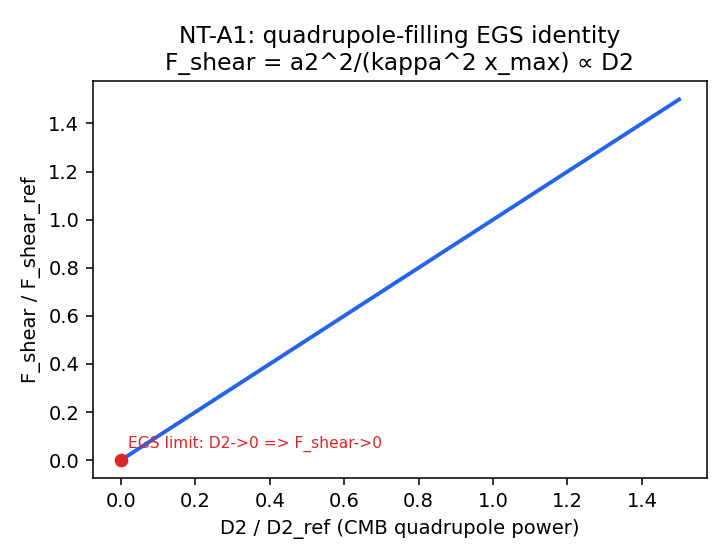
\includegraphics[width=0.70\textwidth]{current/fig_theorem_nt_a1_quadrupole_filling}
\caption{Theorem~\ref{thm:nt-a1} (NT-A1): the shear filling fraction
is linear in the CMB quadrupole power $D_2$ and vanishes in the EGS
limit $D_2\to0$. Diagnostic-only analytic illustration; not a
detection.}
\label{fig:nt-a1}
\end{figure}

\begin{figure}[ht]
\centering
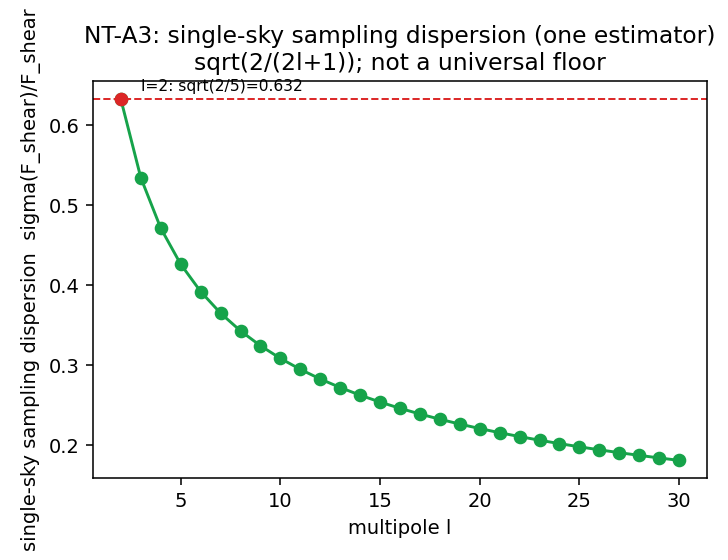
\includegraphics[width=0.70\textwidth]{current/fig_theorem_nt_a3_cosmic_variance_floor}
\caption{Theorem~\ref{thm:nt-a3} (NT-A3): the cosmic-variance
fractional floor $\sqrt{2/(2\ell+1)}$ on $\Fshear$, equal to
$\sqrt{2/5}\approx0.632$ at the quadrupole. Diagnostic-only; not a
detection.}
\label{fig:nt-a3}
\end{figure}

\begin{figure}[ht]
\centering
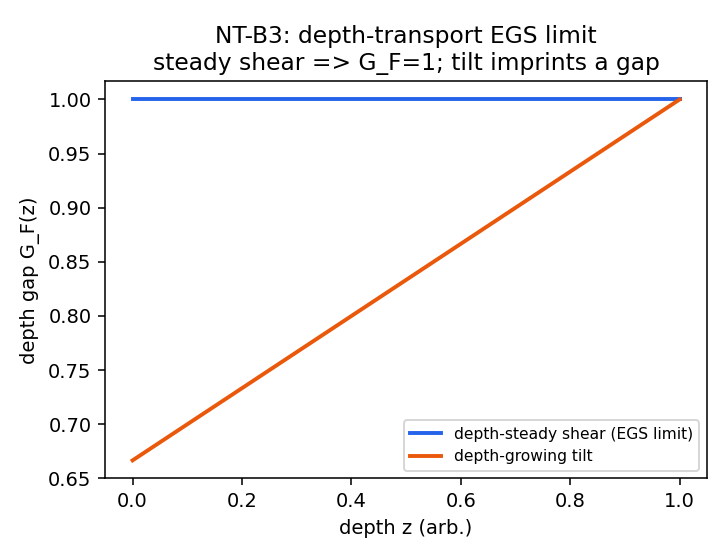
\includegraphics[width=0.70\textwidth]{current/fig_theorem_nt_b3_gf_transport}
\caption{Theorem~\ref{thm:nt-b3} (NT-B3): the depth gap $\GF(z)$ is
flat at unity for a depth-steady shear (EGS depth limit) and rises
when a depth-evolving tilt is present. Diagnostic-only; not a
detection.}
\label{fig:nt-b3}
\end{figure}

\paragraph{Broader conditional-theorem registry.}
A wider set of program theorems (labelled B4, G2, G5, S1, S3, S4,
S5) carries kinetic-theory and information-bound statements onto the
same variables. These are recorded as \emph{convention-conditional}
or \emph{program} theorems whose observational use is blocked by
explicit kill-switches (e.g.\ a nonpositive collision gap blocks any
exponential-forgetting language; a near-zero source rank blocks any
inverse-source claim). They are synthetic/manufactured verification
only and are not promoted to observational results here; the
auditable registry is
\texttt{docs/generated/theorem\_extension\_registry.json}.

% ============================================================
\section{Model-independent real-data measurements}
\label{sec:measurements}

Two genuinely new measurements are produced from real data already
in the repository, using the existing observer-side estimator stack.
Both are model-independent and diagnostic-only: each is calibrated
against a null or resampling baseline, and neither produces a
Bianchi-family, geometry, native-solver, posterior, or certificate
claim.

\subsection{K1 --- Null-calibrated low-$\ell$ morphology of the real Planck map}
\label{sec:k1}

We summarise the Planck PR3 SMICA temperature map at NSIDE$=16$ with
a set of low-$\ell$ scalar and morphology statistics, and calibrate
each against an isotropic $\Lambda$CDM \texttt{synfast} null ensemble
($n=10000$, seed $12345$, CAMB reference spectrum). Table~\ref{tab:k1}
gives the observed values and the null tail probabilities.

\begin{table}[ht]
\centering
\caption{K1: null-calibrated low-$\ell$ statistics of the Planck PR3
SMICA NSIDE$=16$ map. $p$ is the tail probability against the
isotropic $\Lambda$CDM null ($n=10000$). Look-elsewhere across the
six statistics is tracked, not globally corrected.}
\label{tab:k1}
\begin{tabular}{lrrl}
\toprule
Statistic & Observed & $p$ & Tail \\
\midrule
$S_{1/2}$                    & $6.10\times10^{3}$ & $0.059$ & $P(\mathrm{null}\le\mathrm{obs})$ \\
parity even/odd ratio        & $0.628$            & $0.018$ & $P(\mathrm{null}\le\mathrm{obs})$ \\
parity asymmetry             & $-0.228$           & $0.018$ & $P(\mathrm{null}\le\mathrm{obs})$ \\
planarity mean               & $0.518$            & $0.043$ & $P(\mathrm{null}\ge\mathrm{obs})$ \\
$\ell2$--$\ell3$ axis alignment & $69.2^{\circ}$  & $0.65$  & $P(\mathrm{null}\le\mathrm{obs})$ \\
axis-to-CMB-dipole apex      & $72.9^{\circ}$     & $0.71$  & $P(\mathrm{null}\le\mathrm{obs})$ \\
\bottomrule
\end{tabular}
\end{table}

\paragraph{Findings.} The map recovers the parity (odd-power excess,
$p=0.018$) and large-angle ($S_{1/2}$, $p=0.059$) low-$\ell$
anomalies as model-independent, null-calibrated features; planarity
is marginal ($p=0.043$). The power-inertia $\ell2$--$\ell3$ axis and
the axis-to-CMB-apex angle show \emph{no} anomaly in this estimator
($p\approx0.65,0.71$); these are honest nulls, and this is not the
multipole-vector ``axis-of-evil'' statistic. The preferred low-$\ell$
axis lies at Galactic $(l,b)=(326.6^{\circ},-1.0^{\circ})$. Because
the look-elsewhere effect across the six statistics is tracked but
not globally corrected, the parity $p=0.018$ over six trials is not
globally significant. No Bianchi or source-identification claim is
made. The map is full-sky cleaned with no mask deconvolution or full
pixel--pixel covariance.

\begin{figure}[ht]
\centering
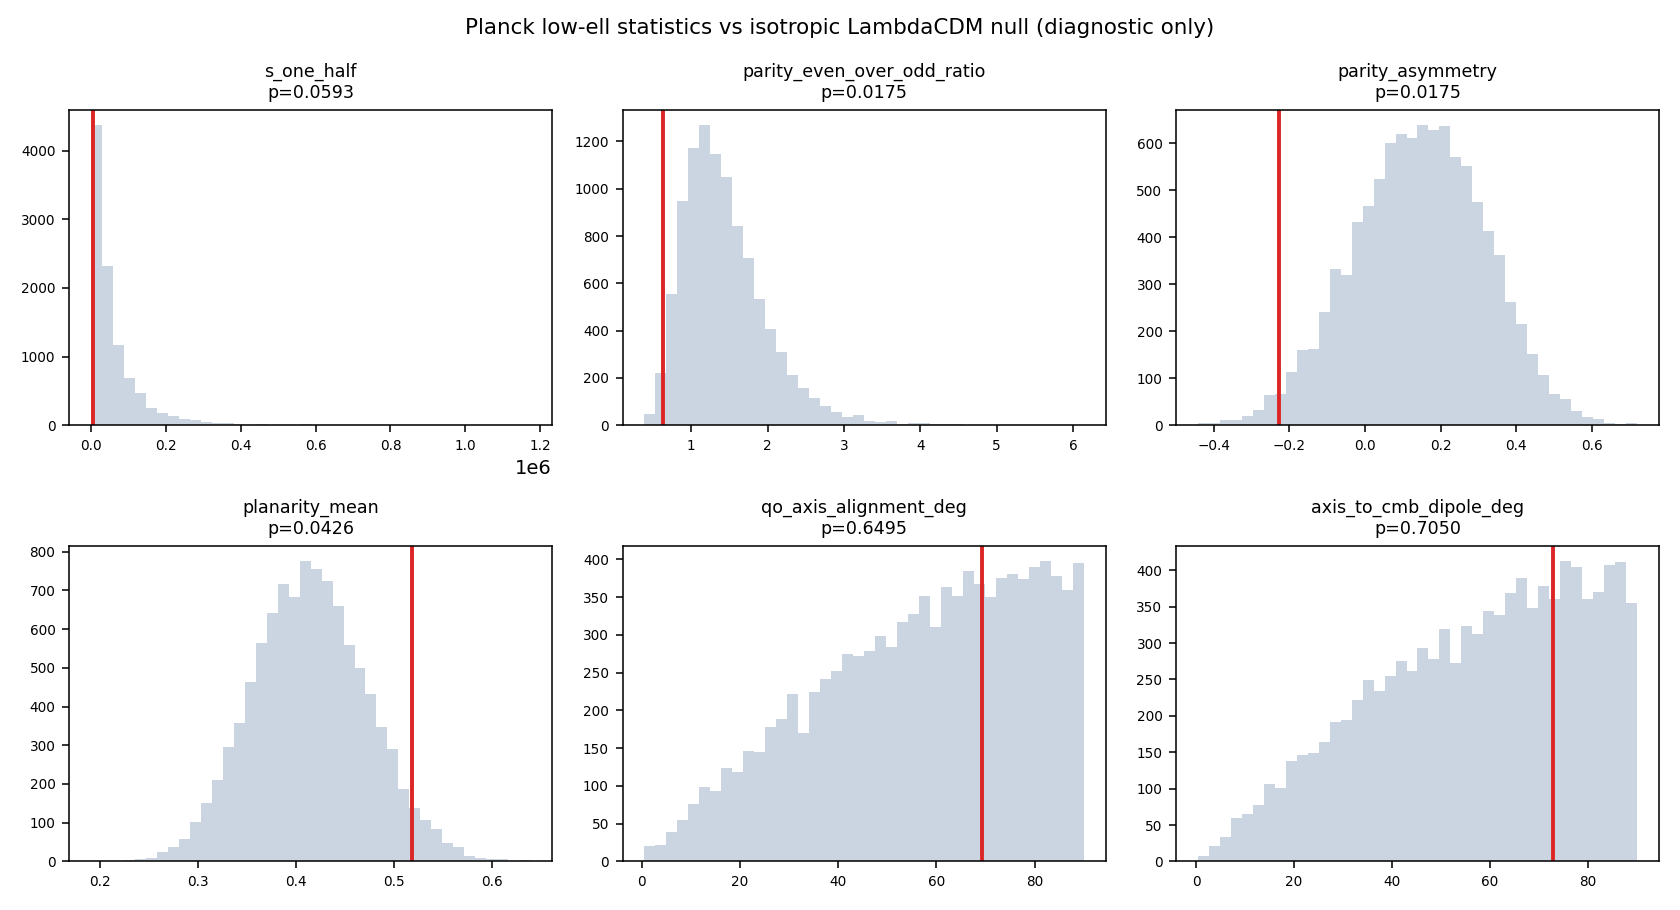
\includegraphics[width=0.78\textwidth]{observed_current/fig_observed_lowell_null_significance}
\caption{K1: observed low-$\ell$ statistics of the Planck PR3 map
against the isotropic $\Lambda$CDM null ensemble. Model-independent
null-calibrated features; not evidence for any Bianchi model.}
\label{fig:k1-sig}
\end{figure}

\begin{figure}[ht]
\centering
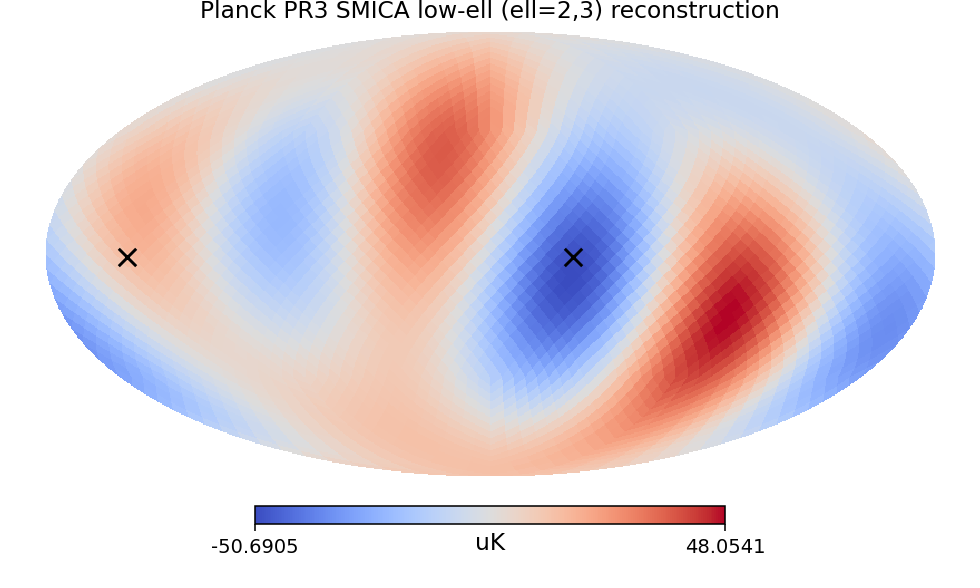
\includegraphics[width=0.78\textwidth]{observed_current/fig_observed_lowell_morphology_axis}
\caption{K1: the power-inertia low-$\ell$ ($\ell=2,3$) preferred axis
of the real Planck map. The axis-alignment and axis-to-apex angles
are null (Table~\ref{tab:k1}). Diagnostic-only; a power-inertia-axis
descriptor, not the multipole-vector axis-of-evil statistic.}
\label{fig:k1-axis}
\end{figure}

\subsection{K4 --- CF4++ bulk-flow apex versus depth}
\label{sec:k4}

From the Cosmicflows-4 (CF4) reconstruction grid we measure the
volume-averaged bulk-flow amplitude and apex direction in seven
radial shells. Table~\ref{tab:k4} gives the profile.

\begin{table}[ht]
\centering
\caption{K4: CF4++ bulk-flow apex by depth shell. $|B|$ is the
volume-averaged reconstruction velocity per shell; the bracketed
figures are bootstrap apex dispersion over correlated reconstruction
cells (a lower bound on direction uncertainty, not a full
covariance). Full-sample bulk flow: $133.4$\,km/s toward
$(l,b)=(121.6^{\circ},70.8^{\circ})$.}
\label{tab:k4}
\begin{tabular}{lrrll}
\toprule
$r$ [Mpc/h] & $N$ cells & $|B|$ [km/s] & apex $(l,b)$ [deg] & to CMB apex [deg] \\
\midrule
$90$--$150$  & $6749$  & $378$ & $(300,24)$  & $36.9$  \\
$150$--$200$ & $10254$ & $531$ & $(301,63)$  & $25.3$  \\
$200$--$250$ & $16091$ & $584$ & $(239,88)$  & $39.9$  \\
$250$--$300$ & $21788$ & $588$ & $(133,75)$  & $52.5$  \\
$300$--$350$ & $27890$ & $222$ & $(114,48)$  & $80.4$  \\
$350$--$400$ & $35806$ & $128$ & $(114,-49)$ & $160.6$ \\
$400$--$450$ & $45179$ & $186$ & $(120,-78)$ & $147.5$ \\
\bottomrule
\end{tabular}
\end{table}

\paragraph{Findings.} The bulk-flow amplitude rises to
$\sim590$\,km/s at $250$--$300$\,Mpc/h and then falls to
$\sim130$--$190$\,km/s in the deep shells. The apex stays within
$\sim5$--$46^{\circ}$ of the full-sample apex out to $300$\,Mpc/h and
then reverses ($\sim120$--$149^{\circ}$) at the reconstruction edge;
the reversal is flagged as a likely edge effect of the
reconstruction. This is a model-independent kinematic descriptor of
the reconstruction; it is not a cosmological-frame-violation or
Bianchi claim, and the bootstrap dispersion is a lower bound on the
true direction uncertainty rather than a full covariance.

\begin{figure}[ht]
\centering
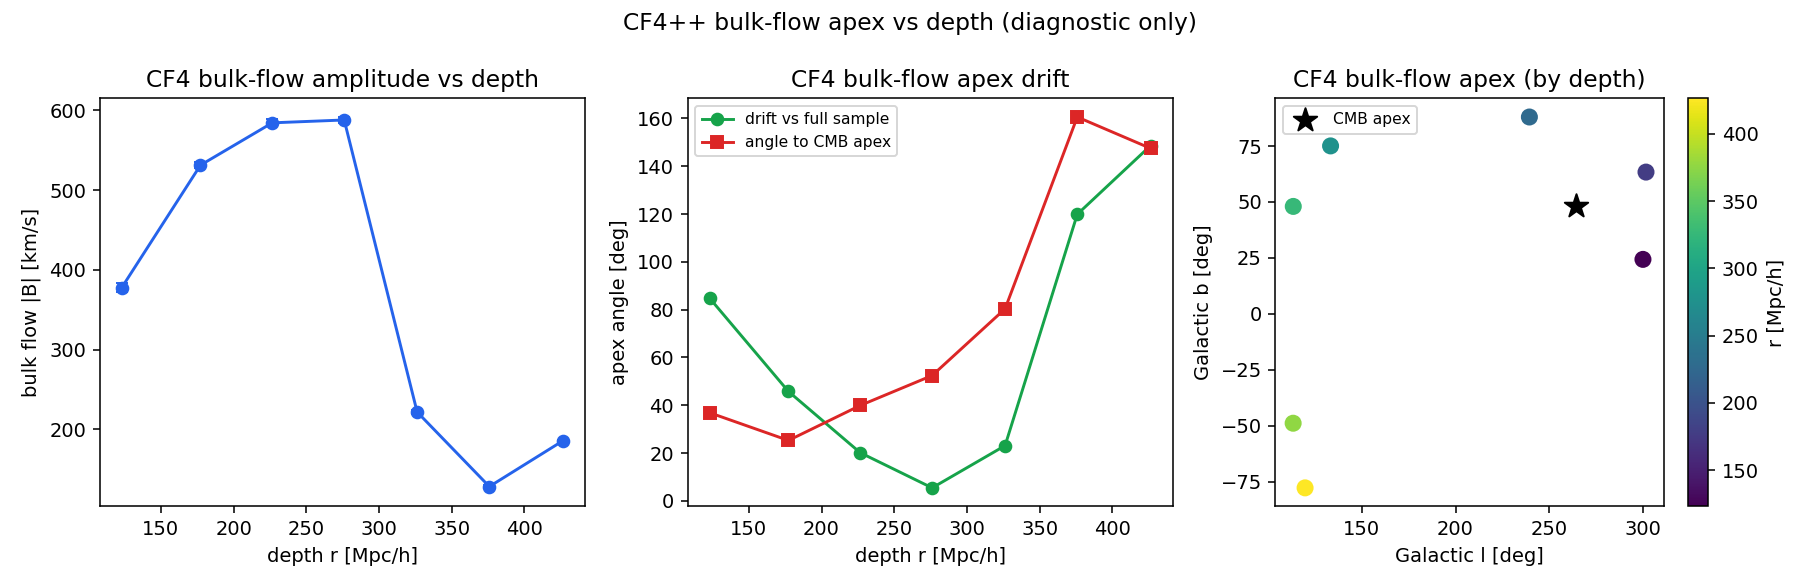
\includegraphics[width=0.82\textwidth]{observed_current/fig_observed_cf4_bulkflow_apex_depth}
\caption{K4: CF4++ bulk-flow amplitude and apex drift versus depth
shell. Model-independent kinematic descriptor; not a frame-violation
or Bianchi claim.}
\label{fig:k4}
\end{figure}

\paragraph{Critically excluded candidates.} Several nearby analyses
were considered and \emph{excluded} as empty or as
re-presentations, to keep this report free of non-results: a joint
common-axis posterior over the four dipoles (the available latent
likelihood has no directional term, so the axis is prior-flat); the
DESI footprint resultant-dipole ``systematics floor'' (already
shipped as a long-run jackknife diagnostic); the DESI cosmological
clustering dipole (blocked: no matched randoms/masks); and any
positive Bianchi/tilt evidence (blocked: amplitude-matched
contamination null, no native morphology atlas).

% ============================================================
\section{Transfer-conditional diagnostics}
\label{sec:transfer}

A separate family of result surfaces depends on \emph{external} or
\emph{empirical-proxy} transfer functions (AniCLASS-external and an
empirical shear$\to D_\ell$ proxy). These are \emph{transfer-conditional}
diagnostics: they are not native low-$\ell$ solver output, they carry
no passed native-validation gate, and the family labels attached to
them are provenance labels only, not classification claims. Any
amplitude-ranking quantity computed along these paths (for example a
configured likelihood-ratio summary for an admitted dipole-amplitude
premise) is a premise-conditioned amplitude fit and a
transfer-conditional ranking; it is prior- and
error-budget-sensitive, it is not a source-identification claim, and
the source origin is not established. The auditable inventory of
transfer dependence is
\texttt{docs/generated/transfer\_sensitivity\_report.md}; the
calibration window for the external shear$\to D_2$ path is the legacy
Saadeh-linear regime $\Sigma^2\in[10^{-24},10^{-20}]$. These rows are
included for completeness and provenance, not as headline results.

% ============================================================
\section{What is not claimed (standing blocks)}
\label{sec:blocks}

For the avoidance of doubt, the following are \emph{not} results of
this report and remain blocked:
\begin{itemize}[leftmargin=1.4em,itemsep=2pt]
  \item an identified Bianchi family or a detected anisotropic
        geometry from any scalar, axis, or low-$\ell$ feature above;
  \item native-solver validation for any external/proxy transfer
        output;
  \item any MIO observatory certificate used as a posterior, a
        truth certificate, a model weight, or an HTT evidence term;
  \item any low-$\ell$ or velocity feature above promoted from a
        model-independent measurement into anisotropy evidence;
  \item a globally significant low-$\ell$ anomaly detection (the
        K1 $p$-values are local, look-elsewhere-tracked, single-sky,
        and not full-covariance/mask-coupled).
\end{itemize}

% ============================================================
\section{Reproducibility}
\label{sec:repro}

Every result above is regenerated by a recorded command and ships a
manifest with input hashes and a claim tier. The load-bearing
artifacts are:
\begin{itemize}[leftmargin=1.4em,itemsep=2pt]
  \item \textbf{Theorems:}
        \texttt{python scripts/prove\_egs\_lowell\_theorems.py}
        $\to$ \texttt{docs/generated/egs\_lowell\_theorem\_proofs.json};
        figures via
        \texttt{python scripts/make\_egs\_lowell\_theorem\_figures.py}.
  \item \textbf{K1 (Planck):}
        \texttt{python scripts/make\_lowell\_morphology\_real\_map.py}
        $\to$ \texttt{docs/generated/lowell\_morphology\_real\_map\_report.\{json,md\}}.
  \item \textbf{K4 (CF4):}
        \texttt{python scripts/make\_cf4\_bulkflow\_apex\_depth.py}
        $\to$ \texttt{docs/generated/cf4\_bulkflow\_apex\_depth\_report.\{json,md\}}.
  \item \textbf{Transfer inventory:}
        \texttt{python scripts/generate\_transfer\_sensitivity\_report.py}.
\end{itemize}
Each figure in this report has a sidecar
\texttt{*.manifest.json} recording owner, claim tier (\emph{diagnostic-only}),
\texttt{family\_identification:false}, and
\texttt{native\_solver\_result:false}.

% ============================================================
\begin{thebibliography}{9}
\small
\bibitem{egs1968} J.~Ehlers, P.~Geren, R.~K.~Sachs,
  ``Isotropic Solutions of the Einstein--Liouville Equations,''
  \emph{J.\ Math.\ Phys.} \textbf{9}, 1344 (1968).
\bibitem{sme1995} W.~R.~Stoeger, R.~Maartens, G.~F.~R.~Ellis,
  ``Proving Almost-Homogeneity of the Universe: An Almost
  Ehlers--Geren--Sachs Theorem,'' \emph{Astrophys.\ J.}
  \textbf{443}, 1 (1995).
\bibitem{mes1995} R.~Maartens, G.~F.~R.~Ellis, W.~R.~Stoeger,
  ``Limits on anisotropy and inhomogeneity from the cosmic
  background radiation,'' \emph{Phys.\ Rev.\ D} \textbf{51}, 1525
  (1995).
\bibitem{etm} J.~Ehlers, R.~Treciokas (and the
  Ehlers--Treciokas--Matravers $\ell=2$ free-streaming closure used
  for $\kappa=4/21$); see also R.~Treciokas, G.~F.~R.~Ellis,
  ``Isotropic solutions of the Einstein--Boltzmann equations,''
  \emph{Commun.\ Math.\ Phys.} \textbf{23}, 1 (1971).
\bibitem{ellisvanelst} G.~F.~R.~Ellis, H.~van Elst,
  ``Cosmological models (Carg\`ese lectures 1998),'' in
  \emph{Theoretical and Observational Cosmology}, NATO ASI
  \textbf{541}, 1 (1999), arXiv:gr-qc/9812046.
\bibitem{fixsen2009} D.~J.~Fixsen,
  ``The Temperature of the Cosmic Microwave Background,''
  \emph{Astrophys.\ J.} \textbf{707}, 916 (2009).
\bibitem{planck2018vii} Planck Collaboration,
  ``Planck 2018 results. VII. Isotropy and statistics of the CMB,''
  \emph{Astron.\ Astrophys.} \textbf{641}, A7 (2020).
\bibitem{cf4} R.~B.~Tully \emph{et al.},
  ``Cosmicflows-4,'' \emph{Astrophys.\ J.} \textbf{944}, 94 (2023).
\end{thebibliography}

\end{document}
